

\chapter{为越南高等教育提出混合与适应性质量保障模型(V-AQA模型)}
\label{chap:de_xuat_vqa}

\section[引言]{引言:背景与新模型的紧迫性}
\addcontentsline{toc}{section}{引言}

基于第三章对越南高等教育质量保障体系现状及其系统性挑战的深入分析,得出了一个重要结论:现存问题之间存在因果联系,形成了复杂的“恶性循环”。世界银行的诊断报告已明确指出治理薄弱、培养与市场脱节以及质量保障体系尚未真正有效等问题\footcite{worldbank_improvingperformance}。这些问题并非孤立存在,而是相互交织,包括:大学自主权仍然有限\footcite{world-bank_improvingperformance},利益相关者参与度不高\footcite{pmc_article_9127449},质量文化带有浓厚的应付色彩\footcite{vjol_reactiveculture},以及质量保障人力资源既缺又弱\footcite{pmc_article_9127449}。

这表明,采用零散、片面的解决方案或机械地照搬国外的传统模式,将无法从根本上解决问题。越南需要一种新的方法,一个全面的行动框架,既能适应一个转型期经济体的特殊背景,又能与国际质量标准接轨。

为响应这一要求,本章将提出并详细论证一个新模型——\textbf{混合与适应性质量保障模型(简称V-AQA)}。该模型不仅是一系列孤立解决方案的集合,更是一个系统的思维和行动框架,旨在直接打破已指出的“恶性循环”,并从内部推动一种可持续的质量文化。

\section{越南现行质量保障框架的差距分析}
\label{sec:phan_tich_khoang_trong}

为申明V-AQA模型的紧迫性和适用性,首先需要分析在越南普遍应用的现有质量保障框架未能彻底解决的差距。

\subsection{东盟大学网络质量保障标准}

东盟大学网络及其质量保障标准在推动质量文化和区域一体化方面做出了巨大贡献。

\paragraph{优势} 东盟大学网络质量保障提供了一套全面的标准(4.0版共8项标准),重点关注成果导向教育和以学习者为中心\footcite{AUN-QAGuide}。获得东盟大学网络质量保障标准认证有助于越南的培养项目提升声誉,并为区域内的学生交换和学分互认创造便利条件\footcite{hoasen_benefits_aunqa}。

\paragraph{差距与局限}
\begin{itemize}
    \item \textbf{主要集中于课程层面:} 尽管有机构层面的标准,但在越南应用东盟大学网络质量保障标准主要发生在课程层面。这可能导致质量不均衡的状况,即少数几个项目达到国际标准,而整个机构,特别是在治理和资源分配方面,仍然沿用旧模式\footcite{aun_institutional_v2}。
    \item \textbf{流程复杂且成本高昂:} 寻求东盟大学网络质量保障认证需要大量的财政和人力资源,这为许多学校,特别是民办或地方院校设置了障碍\footcite{stdjssh_637}。
    \item \textbf{“形式化合规”的风险:} 获得认证的压力可能导致学校专注于完善档案和证据,以机械地满足标准,而不是从内部推动实质性改进\footcite{pmc_article_9127449}。
\end{itemize}

\subsection{教育培训部的规定}
教育培训部的法规文件体系,特别是关于质量认证的通知(如基于东盟大学网络质量保障标准制定的第12/2017号通知),为质量保障活动创造了强制性的法律走廊。

\paragraph{优势} 教育培训部的规定在整个体系内设立了最低质量要求,迫使教育机构进行自评和外部认证,有助于提升对质量保障的普遍认识。

\paragraph{差距与局限}
\begin{itemize}
    \item \textbf{体系缺乏独立性:} 各教育质量认证中心仍受教育培训部的直接管理,这引发了关于国家管理机构与专业认证机构之间客观性和独立性的担忧\footcite{ncdt_journal_219}。
    \item \textbf{大学自主权仍然有限:} 尽管自主政策已经颁布,但执行中仍存在诸多障碍。根据世界银行的报告,只有一小部分公立大学真正参与了自主试点,且自主范围仍然狭窄,特别是在组织和人事方面\footcite{world-bank_improvingperformance}。这降低了学校根据自身需求灵活改进质量的能力。
    \item \textbf{合规文化:} 按照教育培训部规定进行的认证通常被视为一项必须完成的行政义务,导致了“应付式合规”文化,而非内在的改进需求\footcite{vjol_reactiveculture}。
\end{itemize}

\subsection{构思-设计-实现-运作能力框架}
构思-设计-实现-运作是一个先进的框架,被越南许多工科院校采用,以改革培养方案,使其满足企业要求。

\paragraph{优势} 构思-设计-实现-运作提供了一个集成的学习框架,将理论与实践相结合,帮助学生全面发展个人、沟通和专业技能。应用构思-设计-实现-运作极大地推动了工科院校教学方法的创新\footcite{vietnamplus_cdio_reform}。

\paragraph{差距与局限}
\begin{itemize}
    \item \textbf{范围狭窄且难以推广:} 构思-设计-实现-运作主要为工程和技术学科设计。将该模型应用于社会科学、经济学或师范等学科是一个巨大挑战。
    \item \textbf{要求深刻的文化变革:} 成功实施构思-设计-实现-运作要求在思维和组织文化上发生重大变革,从领导层到每一位教师。在越南的研究已指出这种变革的困难,包括初期领导层缺乏正式承诺以及核心教师团队与其余人员之间互动有限\footcite{nguyen_cdio_2016}。
\end{itemize}

\section{V-AQA模型的定位:比较优势与优越性}
\label{sec:dinh_vi_vqa}

基于对上述差距的分析,提出V-AQA模型并非旨在完全替代,而是为了整合并克服现有框架在越南特殊背景下未能彻底解决的固有弱点。

与这些模型相比,V-AQA拥有突出的优势:
\begin{itemize}
    \item \textbf{混合性:} 主动平衡来自外部的\textbf{问责制}压力(教育培训部的要求)和来自内部的\textbf{持续改进}动力(东盟大学网络质量保障和构思-设计-实现-运作的精神),而不是只关注一个方面。
    \item \textbf{适应性:} 按照灵活的短期改进周期运作,帮助学校快速响应市场变化,而不是遵循僵化的长期计划。
    \item \textbf{全面性与内生性:} 作用于学校的全部五个核心方面(领导与治理、文化、利益相关者、流程、合作),并推动来自内部的变革(内生性),而不仅仅是遵守外部要求。
    \item \textbf{技术整合性:} 以管理信息系统为“神经系统”,使基于证据的治理成为可能,这是其他框架未直接提及的因素。
\end{itemize}

为更清晰地说明这种差异,下表将V-AQA与越南普遍应用的框架进行对比:

\begin{table}[h!]
\centering
\caption{V-AQA模型与普遍应用框架的对比表}
\label{tab:doi_sanh_vqa}
\begin{tabular}{|p{3cm}|p{3.5cm}|p{3.5cm}|p{3.5cm}|}
\hline
\textbf{比较标准} & \textbf{东盟大学网络质量保障(课程层面)} & \textbf{教育培训部规定(第12号通知)} & \textbf{V-AQA模型(建议)} \\
\hline
\textbf{主要目标} & 根据东盟共同标准评估、比对课程质量。 & 为各校规定最低标准和强制性认证流程。 & \textbf{从内部创建一个全面、自我改进且可持续的质量体系。} \\
\hline
\textbf{应用范围} & 主要在培养课程层面。 & 课程层面和教育机构层面。 & \textbf{全面覆盖学校层面,从领导、文化到每一个流程。} \\
\hline
\textbf{自主程度} & 学校自愿参加,但必须严格遵守东盟大学网络流程。 & 低,认证机构仍依赖教育培训部,合规性强\footcite{ncdt_journal_219}。 & \textbf{高且有导向:推动自主与通过关键绩效指标明确问责相结合。} \\
\hline
\textbf{利益相关者参与} & 有提及,但实际上学生和企业参与仍然有限\footcite{pmc_article_9127449}。 & 咨询性质,缺乏实质性约束机制。 & \textbf{将利益相关者的角色机制化(行业咨询委员会、学术委员会中的学生代表)。} \\
\hline
\textbf{灵活性} & 标准化流程,灵活性低。 & 规定具有普遍适用性,较为僵化。 & \textbf{高,是核心原则(适应性),允许根据短期周期进行调整。} \\
\hline
\end{tabular}
\end{table}

\textit{(注:构思-设计-实现-运作能力框架未直接纳入比较表,因为其本质是针对工科领域的专门培养方案开发框架,与东盟大学网络质量保障和教育培训部规定的综合性质量保障体系性质不同)。}

上表显示,V-AQA不仅是一套标准,更是一个\textbf{治理框架}。V-AQA不只关注“需要达成什么”,更关注“如何”构建一个能够自我改进的组织。这种方法直接解决了自主、质量文化和利益相关者参与等基础性问题,而仅仅应用单一标准是无法触及这些问题的。

为更深入地理解塑造这些比较优势的思想基础,下一部分将深入论证V-AQA模型的混合理念与适应性原则。


% het goi 1


\section{V-AQA模型的哲学基础与原则}
\label{sec:triet_ly_nguyen_tac_vqa}

V-AQA模型建立在两大哲学基础上,这两大基础是从国际研究和对越南特殊背景的分析中总结出来的:混合哲学与适应性原则。这正是该模型的“灵魂”,塑造了其所提出的方法和解决方案。

\subsection{混合哲学:协调问责制与质量改进}

越南高等教育体系目前正承受着双重压力。一方面,由于国家的主导作用和对公共预算的依赖,各大学必须强有力地满足\textbf{问责制}的要求。另一方面,在日益激烈的竞争和劳动力市场要求的背景下,各大学又迫切需要进行\textbf{改进}以提升质量和品牌。

这两个目标常常产生矛盾,导致要么过分注重形式上的合规以满足外部要求,要么是自发、无纪律的内部改进。V-AQA模型的“混合”哲学正是为了解决这种紧张关系而提出的。正如哈维和威廉姆斯(2010)在对高等教育质量十五年的综述中所分析的,一个有效的体系必须设法整合并协调这两个目标\footcite{harvey_williams_2010}。V-AQA模型通过承认外部透明的问责要求可以为推动内部改进努力提供必要的数据和压力来实现这一点。反之,强大的改进文化将使学校更容易满足并超越问责要求。这种方法有助于将关系从对抗转为共生,其中遵守规定成为前提,而提升质量成为最终目标。

\subsection{适应性原则:在变化背景下的灵活性}

越南的经济社会和政策背景正在以极快的速度变化。第四次工业革命、关于大学自主的新政策以及劳动力市场的波动,都要求质量保障体系必须具有高度的灵活性。一个为期五年的僵化质量改进计划,有可能在尚未执行完毕时就已经过时。

因此,V-AQA模型建立在“适应性”原则之上,其灵感来自于像适应性项目框架这样的敏捷项目管理框架\footcite{Wysocki2009}。该原则鼓励采用短期的、重复的改进周期,而不是一个长期的PDCA循环。各学校可以按学年甚至学期设定质量目标,实施、快速收集反馈数据,并为下一个周期调整计划。这种方法帮助各学校“边做边学”,最大限度地减少长期错误决策的风险,并确保改进努力始终与不断变化的实际背景相符。

\section{V-AQA模型的总体结构与要素}
\label{sec:cau_truc_tong_the}

基于上述两大哲学基础,V-AQA模型被建构为一个由理论基础、五个相互作用的核心要素和最终目标组成的总体结构。

\begin{figure}[h!]
    \centering
    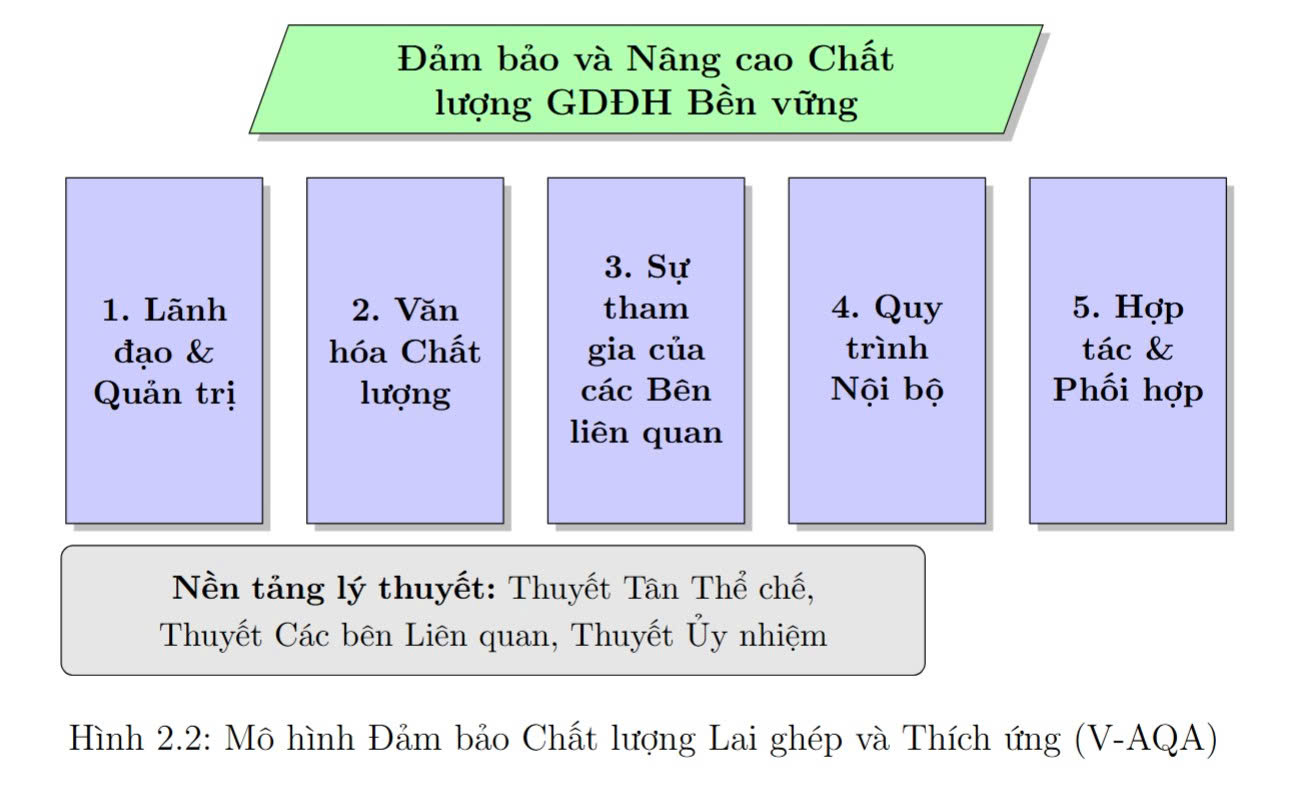
\includegraphics[width=\textwidth]{image/mo_hinh_V-AQA.jpg}
    \caption{混合与适应性质量保障模型 (V-AQA)}
    \label{fig:v-aqa-model-detailed}
\end{figure}

V-AQA模型的五个要素相互作用,形成一个完整的质量体系。为给读者,特别是那些非质量保障领域的专业人士,提供一个全面且易于理解的概览,下表将总结每个要素的目标、具体表现以及建议的关键绩效指标。该表如同一张“地图”,为后续的详细分析部分勾画了结构。

\begin{longtable}{|p{2.5cm}|p{3.5cm}|p{4.5cm}|p{3.5cm}|}
\caption{V-AQA模型5要素总结}
\label{tab:tong_hop_5_thanh_to}\\
\hline
\textbf{要素} & \textbf{主要目标} & \textbf{具体表现(行动)} & \textbf{衡量方式(关键绩效指标示例) \footcite{uq_kpi_dashboard}} \\
\hline
\endfirsthead
\multicolumn{4}{c}%
{{\bfseries \tablename\ \thetable{} -- 续前页}} \\
\hline
\textbf{要素} & \textbf{主要目标} & \textbf{具体表现(行动)} & \textbf{衡量方式(关键绩效指标示例) \footcite{uq_kpi_dashboard}} \\
\hline
\endhead
\hline \multicolumn{4}{r}{{续下页}} \\
\endfoot
\hline
\endlastfoot

% 第1行
\textbf{1. 领导与治理} & 将领导者从“控制者”转变为“环境创造者”。 & 
\begin{itemize}
    \item 制定并执行校级质量战略。
    \item 向院系下放强有力的权力并辅以问责制。
    \item 为中层管理团队提供能力提升培训。
\end{itemize} & 
\begin{itemize}
    \item 质量战略中各项目标的完成率。
    \item 各院系对自主权的满意度。
    \item 完成现代治理培训的中层管理者数量。
\end{itemize} \\
\hline

% 第2行
\textbf{2. 质量文化} & 从“应付式合规”文化转变为“主动改进”文化。 & 
\begin{itemize}
    \item 发起系统的质量宣传运动。
    \item 建立表彰和奖励改进创举的体系。
    \item 成立并授权“质量改进小组”。
\end{itemize} & 
\begin{itemize}
    \item 关于质量文化认知的定期调查得分。
    \item 每年提出并实施的改进创举数量。
    \item 参与改进活动的教职工比例。
\end{itemize} \\
\hline

% 第3行
\textbf{3. 利益相关者的参与} & 将利益相关者(企业、学生、校友)转变为“战略伙伴”。 & 
\begin{itemize}
    \item 将行业咨询委员会的活动机制化。
    \item 让学生代表在科学与培养委员会中拥有投票权。
    \item 建立主动的“校友大使”网络。
\end{itemize} & 
\begin{itemize}
    \item 行业咨询委员会的建议被整合到培养方案中的比例。
    \item 有学生代表参与的学术决策数量。
    \item 企业对毕业生契合度的满意度得分。
\end{itemize} \\
\hline

% 第4行
\textbf{4. 内部流程} & 基于数据实现学术和管理流程的现代化、标准化。 & 
\begin{itemize}
    \item 采用基于成果导向教育理念的培养方案开发流程。
    \item 多样化教学和评估方法。
    \item 构建并整合质量保障管理信息系统。
\end{itemize} & 
\begin{itemize}
    \item 按照成果导向教育流程制定和审查的培养方案比例。
    \item 课程中过程性评估分数的平均比重。
    \item 基于质量保障管理信息系统数据做出的管理决策比例。
\end{itemize} \\
\hline

% 第5行
\textbf{5. 合作与协调} & 打破“孤岛”状态和封闭思维,创造一个开放的质量生态系统。 & 
\begin{itemize}
    \item 为跨学科、跨单位的质量改进项目提供经费。
    \item 建立并参与标杆比对网络。
    \item 战略性地利用国际认证活动进行学习。
\end{itemize} & 
\begin{itemize}
    \item 成功实施的跨院系/部门项目数量。
    \item 组织的标杆比对活动及产生改进报告的数量。
    \item 国际认证建议的完成比例。
\end{itemize} \\
\end{longtable}

本章的后续部分将深入分析和论证上述五个要素中的每一个,包括建议的解决方案、科学依据、潜在风险及缓解策略。



% het goi 2 chuong 4



\section{V-AQA模型的各要素与建议解决方案}
\label{sec:cac_thanh_to_vqa}

V-AQA模型由五个相互作用的要素构成,每个要素代表一组战略性解决方案,旨在解决第三章中已分析的挑战。接下来的部分将深入探讨每个要素,论证其建议的解决方案及其背后的科学与实践依据。

\subsection{要素一:以分权和责任为导向重构领导与治理}
\label{subsec:giaiphap_lanhdao}

如前所述,当前质量保障体系的最大障碍之一是领导角色带有浓厚的行政、合规色彩,且权力过于集中\footcite{vnujs_fs_4303}。因此,V-AQA模型的第一个要素聚焦于重构这一角色,目标是将领导者从“控制者”转变为质量文化的“环境创造者”和“推动者”\footcite{unesco_gem_report_2024}。

\paragraph{解决方案1.1:制定并执行校级质量战略。}
为摆脱季节性的应付状态,每所大学都需要制定一份正式的五年期\textbf{质量战略},并将其紧密融入学校的总体发展战略中。这并非一份形式化的文件,而是最高层领导的政治承诺。该战略必须回答以下核心问题:
\begin{enumerate}
    \item 学校从哪些维度定义“质量”(研究质量、教学质量、市场契合度、学生体验)?
    \item 未来五年的优先质量目标是什么,并以可衡量的关键绩效指标具体化?(例如:将学生就业率提高到95%,国际发表数量每年增加20%)。
    \item 将分配哪些资源(财政、人力、技术)来实现目标?
    \item 谁为每个具体目标负责(明确各处、室、院系的角色分工)?
\end{enumerate}
拥有一份清晰且广为宣传的战略,是有效和负责任地执行自主权的先决条件,正如教育培训部关于大学自主的报告所强调的\footcite{moet_report_autonomy}。

\paragraph{解决方案1.2:按“指导核心”模型进行分权并明确授权。}
基于委托代理理论\footcite{JensenMeckling1976},V-AQA模型提出了一种更强有力的分权机制,并辅以明确的问责制。学校需要从集权结构转向克拉克(1998)所分析的“指导核心”模型\footcite{clark_1998}。据此:
\begin{itemize}
    \item \textbf{校董会:} 专注于批准总体战略,监督战略目标的执行,并确保学校对社会的问责。
    \item \textbf{校领导班子:} 负责运营,制定支持性政策,并有效分配资源,以便各单位能够实现目标。
    \item \textbf{各院/系:} 必须在学术事务,如改进培养方案、创新教学方法和开展研究活动等方面,被赋予实质性的自主权。
\end{itemize}
这种自主权必须与一个清晰透明的关键绩效指标体系相结合。校领导班子使用该体系(通过质量保障管理信息系统上的仪表盘)来监督成效,而无需对具体的专业活动进行微观干预,这符合“远程指导”的精神。

\paragraph{解决方案1.3:提升中层管理团队的能力。}
一个好的战略无法由一个薄弱的管理团队来执行。因此,V-AQA模型强调投资于中层管理团队(院/系主任、副主任)能力的必要性。需要设计强制性的培训项目,不仅涉及行政业务,还包括现代大学治理技能,如:
\begin{itemize}
    \item 变革管理
    \item 战略思维与规划
    \item 数据驱动决策
    \item 激励型领导力
\end{itemize}
政府的\textbf{89号提案}等海外博士师资培训项目,应被利用并扩展,以包括为潜在管理者提供关于大学治理的培训和进修项目\footcite{moet_project_89}。这是对“人力资本”的投资,以确保改革从根本上取得成功。

\subsection{领导与治理要素的风险分析与缓解方案}
\label{subsec:risk_lanhdao}
重构领导与治理角色总是潜藏着重大风险。识别并制定预防这些风险的策略是确保成功的关键。

\begin{itemize}
    \item \textbf{风险1:高层领导的承诺浮于表面。}
    \textit{表现:} 领导可能在文件上支持改革,但行动上并不坚决,不提供足够资源,或在遇到困难时轻易改变优先事项。
    \textit{缓解策略:}
    \begin{itemize}
        \item 成立一个由校长或常务副校长直接担任组长的\textbf{质量改革指导委员会},有定期的会议日程和公开的报告。
        \item 为\textbf{校领导班子和各单位领导制定并颁布关键绩效指标},其中执行质量战略的指标在年终评优奖励中占有重要比重。
    \end{itemize}

    \item \textbf{风险2:来自中层管理的抵制。}
    \textit{表现:} 院系主任、处长可能会觉得在一个更透明的体系下运作会失去权力。他们可能会通过不合作、拖延实施或提供不准确的数据来进行暗中抵制。
    \textit{缓解策略:}
    \begin{itemize}
        \item 为100%的中层管理干部组织关于\textbf{变革管理和数据驱动治理的强制性培训},使他们清楚理解新模型的益处。
        \item \textbf{授权与赋能并行。} 当一个院系被分配了更高的关键绩效指标时,也必须在财务和人事方面赋予其相应的自主权,以便能够完成任务。
        \item \textbf{沟通与倾听:} 组织校领导班子与中层管理之间的定期对话会,倾听困难并共同寻找解决方案,而不是单向命令。
    \end{itemize}

    \item \textbf{风险3:分权但无法控制成效。}
    \textit{表现:} 过度下放自主权而没有一个有效的监督体系,可能导致院/系运作偏离方向,无法为学校的总体目标做出贡献。
    \textit{缓解策略:}
    \begin{itemize}
        \item \textbf{部署质量保障管理信息系统是先决条件。} 如果没有一个足够强大的信息系统来为校领导班子提供及时准确的数据,就无法进行分权。
        \item 建立一个\textbf{自上而下统一的、清晰的关键绩效指标体系},确保院/系/处室级别的指标都旨在实现校级战略指标。
    \end{itemize}
\end{itemize}

通过预见并主动管理上述风险,领导与治理要素可以成为强大的动力,而不是障碍,推动整个质量改革进程。


% het goi 3



\subsection{要素二:从合规文化向改进文化的转型}
\label{subsec:giaiphap_vanhoa}

“反应型质量文化”的挑战——即质量保障活动仅为应对外部认证要求而进行——已被确定为阻碍越南大学实质性质量提升的最大障碍之一\footcite{vjol_reactiveculture}。因此,V--AQA模型的第二个要素聚焦于制定战略性解决方案,以创造一个环境,使质量改进成为组织内从领导到员工每个成员的内在需求和日常习惯。

\paragraph{解决方案2.1:基于欧洲大学协会能力框架发起质量文化建设运动。}
文化不能靠命令创造,而必须通过共识和共享价值观来培育。V--AQA模型建议各大学基于\textbf{欧洲大学协会的质量文化框架},开展系统的宣传和意识提升运动\footcite{eua_quality_culture}。根据该能力框架,质量文化建立在机构层面和个人层面因素的互动之上。
\begin{itemize}
    \item \textbf{在机构层面:} 学校领导必须率先垂范,不断宣传质量的愿景、定义和重要性。关于质量的核心价值观必须被整合到发展战略、政策文件和学校的运作流程中。
    \item \textbf{在个人层面:} 运动需要侧重于提升每位教师、员工的意识、态度和能力。具体活动包括:组织研讨会、关于质量思维的培训课程,以及为坦诚对话质量改进中的障碍与机遇而设的开放论坛。
\end{itemize}
该运动的目标是让所有成员明白,质量不仅是质量保障部门的责任,而是每个人的责任。

\paragraph{解决方案2.2:建立改进创举的表彰与奖励体系。}
要将认知转化为行动,需要有实际的激励。V--AQA模型建议建立一个正式的表彰与奖励体系,以嘉奖质量改进的努力。正如哈维和威廉姆斯(2010)所指出的,创建激励机制是维持质量活动的重要组成部分\footcite{harvey_williams_2010}。具体而言,学校可以:
\begin{itemize}
    \item \textbf{设立年度奖项:} “教学创新年度教师奖”、“高效质量保障模式院系奖”、“最佳质量改进创举奖”。这些奖项需要有足够大的物质和精神价值以产生吸引力。
    \item \textbf{融入职业评估与发展流程:} 对质量改进的贡献标准必须被正式纳入年终干部、教师的评估、评级和评优奖励流程中。在规划、任命干部或考虑提前晋升时,这是一个重要的考量因素。
    \item \textbf{公开表彰:} 取得优异成绩的个人和集体需要在学校的宣传渠道(网站、简报、社交媒体)上隆重表彰,以传播良好榜样。
\end{itemize}
这些行动将发出一个强有力的信息:学校真正重视并奖励改进的努力,而不仅仅是看重完成行政任务。

\paragraph{解决方案2.3:通过“改进小组”为教师赋能并建设其能力。}
质量文化必须从基层建立。为解决教师“被动参与”的状况\footcite{iosr_passiveparticipation},V--AQA模型建议授权并创造条件,让他们成为改进过程的主体。具体解决方案是在系或院层面成立\textbf{“质量圈”}。这些是由自愿参加的教师组成的小组,任务是定期讨论教学、研究中的质量问题并提出解决方案。学校需要为这些小组提供小额预算(创举支持基金),以便他们可以试验新的教学方法、开发创新学习材料或组织专业研讨会。这种授权和资源提供将促进一种主人翁精神,将教师从被管理者转变为质量的创造者。

\subsection{质量文化要素的风险分析与缓解方案}
\label{subsec:risk_vanhoa}
改变组织文化是最困难和最长期的挑战之一。实施上述解决方案可能会面临以下风险:

\begin{itemize}
    \item \textbf{风险1:团队的惰性和怀疑态度。}
    \textit{表现:} 教师、员工已习惯于旧的工作方式,认为各种运动和活动只是形式主义,“雷声大雨点小”。他们可能会不情愿地参与,并且不相信会发生实质性变化。
    \textit{缓解策略:}
    \begin{itemize}
        \item \textbf{领导的模范作用:} 领导必须率先参与所有活动,从研讨会到提出创举。领导的行动比任何言语都更有说服力。
        \item \textbf{专注于“速赢”:} 在初期阶段,需要集中支持小型改进小组,以创造出积极、可见的成果。广泛宣传并奖励这些初步成功,将为改革过程创造动力并巩固信心\footcite{kotter_leading_change}。
    \end{itemize}

    \item \textbf{风险2:奖励体系不公平或吸引力不足。}
    \textit{表现:} 奖励评审过程不透明,带有主观性,或者奖励过小,无法产生真正的激励。这可能适得其反,造成不满和嫉妒。
    \textit{缓解策略:}
    \begin{itemize}
        \item \textbf{建立清晰、公开的创举评估标准:} 标准需要能够衡量创举对提升质量的影响(例如:改善学生学习成果,缩短手续办理时间)。
        \item \textbf{多样化奖励形式:} 除了财务奖励,还需要有其他形式的认可,如参加国际培训的机会,在职称评定中优先考虑,或在学校重大活动中获得表彰。
    \end{itemize}

    \item \textbf{风险3:“改进小组”运作效率低下。}
    \textit{表现:} 小组成立后没有实质性活动,只是形式上的会议,或者小组的建议未得到上级的倾听和支持。
    \textit{缓解策略:}
    \begin{itemize}
        \item \textbf{提供必要的资源和支持:} 学校需要设立一个申请和拨付流程简单的“创举支持基金”。同时,需要有一个单位(例如:质量保障处)扮演协调角色,为各小组提供专业支持。
        \item \textbf{建立正式的反馈机制:} 必须有一个清晰的流程,让院/校领导倾听并回应来自改进小组的建议。建议被认真考虑并付诸实施,将是小组继续运作的最大动力。
    \end{itemize}
\end{itemize}

建设质量文化是一场马拉松,而不是短跑。它需要学校各级人员的毅力、一致性和真正的承诺。

% het goi 4 chuong 4



\subsection{要素三:将利益相关者转变为战略伙伴}
\label{subsec:giaiphap_lienquan}

第三章已指出,越南质量保障体系的固有弱点之一是与利益相关者,特别是企业界和学习者本身,缺乏实质性联系\footcite{worldbank_improvingperformance}。这种关系通常停留在形式化、被动的层面,如单向的咨询活动或影响甚微的调查\footcite{vnujs_er_3848}。V-AQA模型的第三个要素提出了旨在打破学校与社会之间“壁垒”的解决方案,将关系从“形式化咨询”转变为“战略合作”。

\paragraph{解决方案3.1:通过咨询委员会将校企联系机制化。}
为使与企业的合作不再依赖于少数领导的个人关系或季节性活动,V-AQA模型提出了一个制度性解决方案:为每个专业或专业群成立并运作\textbf{行业咨询委员会}。这是在东盟大学网络质量保障或ABET等权威国际认证标准中的一项核心要求,这些标准强调利益相关者在设计和改进培养方案中的中心作用\footcite{aunqa_guidelines_v4}。

行业咨询委员会的作用不仅限于参加研讨会。其运作章程需要明确制定,规定具体且具有约束力的任务:
\begin{itemize}
    \item \textbf{审定预期学习成果:} 行业咨询委员会负责审定并对专业院系制定的预期学习成果提出建议,确保其真实反映劳动力市场当前和未来的能力要求(知识、技能、态度)。
    \item \textbf{为培养方案提供定期建议:} 每年至少一次,专业院系必须向行业咨询委员会提交培养方案的审查报告,以获取关于技术、软技能和行业新趋势的更新建议。这些建议必须被记录并有相应的回应计划。
    \item \textbf{参与学术活动:} 邀请行业咨询委员会成员参与毕业设计答辩委员会;在专业课程中担任客座讲师;或为学生提出实际的项目课题。
\end{itemize}
这种机制化将创造一个可持续的对话与合作渠道,确保培养方案始终“跟上”实践,解决培养与市场“不匹配”的问题\footcite{worldbank_improvingperformance}。

\paragraph{解决方案3.2:提升学生和校友的角色。}
除了企业,学生和校友是对一个培养方案质量有最深刻见解的利益相关者。然而,他们通常被视为质量保障体系中的被动对象\footcite{pmc_article_9127449}。V-AQA模型基于阿恩斯坦的“参与阶梯”精神,提出了将他们的角色从被调查对象提升为真正合作伙伴的解决方案\footcite{Arnstein1969}。
\begin{itemize}
    \item \textbf{为学生赋权:} 学生代表(通过民主方式选举产生)不应只参与活动性组织,而应在像院级科学与培养委员会这样的学术性委员会中拥有一个带有\textbf{投票权}的正式席位。这确保了学习者的声音在关于课程、教学方法和学生支持政策等重要决策中得到认真考虑。
    \item \textbf{建立主动的校友网络:} 为每个专业建立一个\textbf{“校友大使”}体系。这些是事业有成且热心的校友,被正式邀请参与为低年级学生提供咨询和职业指导。更重要的是,他们将是定期提供关于培养方案在实际工作中的契合度的结构化反馈的来源。来自学生就业调查的数据\footcite{moet_graduate_survey}将是该网络有效运作的重要输入。
\end{itemize}

\subsection{利益相关者要素的风险分析与缓解方案}
\label{subsec:risk_lienquan}
加强利益相关者的参与,尽管非常必要,但在实施过程中也面临不少风险。

\begin{itemize}
    \item \textbf{风险1:企业参与流于形式,不具实质性。}
    \textit{表现:} 行业咨询委员会成员可能因人情关系而接受邀请,但不花时间研究文件并提出肤浅的建议。他们将此视为一项“社交”活动而非专业责任。
    \textit{缓解策略:}
    \begin{itemize}
        \item \textbf{建立“双赢”关系:} 除了为社会做贡献,学校需要为企业创造实际利益,如:为他们的员工提供进修课程,提供招聘品牌宣传机会,或优先对接研究和技术转让项目。
        \item \textbf{谨慎选择行业咨询委员会成员:} 优先选择真正热心于教育、具有深厚专业知识并愿意承诺时间的专家。行业咨询委员会的运作章程需要有替换不活跃成员的条款。
    \end{itemize}

    \item \textbf{风险2:学生代表的冷漠或能力不足。}
    \textit{表现:} 学生被赋予权力但因胆怯、缺乏批判性思维能力或未被提供足够信息以提出建设性意见而不发言。
    \textit{缓解策略:}
    \begin{itemize}
        \item \textbf{为学生代表组织技能培训课程:} 在参加委员会之前,学生代表需要接受关于批判性思维、如何阅读和分析政策文件以及有效沟通技巧的培训。
        \item \textbf{充分、及时地提供信息:} 委员会会议的材料必须在合理的时间前发送给学生代表,以便他们可以研究并收集其他学生的意见。
    \end{itemize}

    \item \textbf{风险3:利益和观点的冲突。}
    \textit{表现:} 来自企业的建议可能过分集中于眼前的实践技能,轻视基础知识。反之,校方可能固守己见,不愿改变已稳定的培养方案。
    \textit{缓解策略:}
    \begin{itemize}
        \item \textbf{院系/单位负责人的协调作用:} 单位负责人必须扮演“桥梁”角色,有能力协调、分析和融合不同观点,以找到平衡学术与实践要求的最佳解决方案。
        \item \textbf{基于数据做决策:} 所有争论都需要有客观数据的支持,例如就业率数据、校友调查以及劳动力市场趋势分析报告。
    \end{itemize}
\end{itemize}

将利益相关者转变为合作伙伴不仅仅是一个权宜之计,而是一项长期的战略投资。一旦成功,它将创造一个良性循环,其中培养质量不断改进以满足社会的实际需求。

% het goi 5 chuong 4


\subsection{要素四:核心学术流程的现代化}
\label{subsec:giaiphap_quytringnoibo}

为从根本上解决第三章所分析的培养与实践“脱节”问题,改革核心学术流程是一项强制性任务。这些流程正是学校的“生产机器”;如果它们落后,产出产品(毕业生)将难以满足现代社会的要求。因此,V-AQA模型的第四个要素聚焦于两个基础流程的标准化和现代化:(1)培养方案的开发,以及(2)教与学及评估的方法。

\subsubsection{解决方案4.1:采用基于成果导向教育的培养方案开发流程。}
V-AQA模型建议各大学完全转向基于\textbf{成果导向教育}理念的培养方案开发方法。这是东盟大学网络质量保障和ABET等世界上大多数权威认证组织所采用的方法\footcite{aunqa_guidelines_v4}。该理念将重点放在学生毕业后所能达到的成果,而不是仅仅关注需要传授的知识内容。成果导向教育有助于回答“学生能做什么?”这个问题,而不仅仅是“学生知道什么?”。

肤浅地应用成果导向教育,仅仅停留在罗列预期学习成果而没有在整个课程中实现紧密联系,是越南大学正在面临的困难之一\footcite{ijlter_elo_copy}。因此,V-AQA建议一个基于成果导向教育的培养方案开发流程必须包含以下五个紧密相连的步骤:

\begin{enumerate}
    \item \textbf{第一步:利益相关者需求分析。} 流程始于系统地收集和分析来自劳动力市场(通过报告、调查)、行业专家(通过访谈、研讨会)、成功校友和其他利益相关者的要求,以确定学生毕业后所需的能力框架。
    
    \item \textbf{第二步:预期学习成果的制定与审定。} 基于需求分析,专业院系将制定一套清晰、具体、可衡量(SMART)的课程预期学习成果。重要的是,这套预期学习成果必须经过\textbf{行业咨询委员会的审定和建议},以确保其适切性和实践性。
    
    \item \textbf{第三步:设计课程地图。} 这是确保培养方案逻辑性和一致性的关键步骤。构建一个矩阵,清晰地展示课程中的每一门课如何为实现一个或多个预期学习成果做出贡献。这种技术,也被称为“建设性对齐”\footcite{biggs_constructive_alignment},确保了没有任何一门课程是孤立存在的,并且所有的教-学-评活动都指向已确定的预期学习成果。
    
    \item \textbf{第四步:审定与批准。} 设计完成的培养方案(包括预期学习成果、课程地图、各课程详细大纲)必须经过一个权威的委员会(科学与培养委员会,包括外部专家)的审定和批准,然后才能正式颁布。
    
    \item \textbf{第五步:定期审查与改进。} 成果导向教育是一个持续的循环。学校必须建立一个正式的培养方案审查周期(例如:每2-3年一次),基于重要的输入数据,如:来自行业咨询委员会的反馈、毕业生对工作满足度的调查、学生的实际学习成果以及行业的新趋势。
\end{enumerate}

\subsubsection{解决方案4.2:多样化教与学及评估方法。}
一个按照成果导向教育精心设计的培养方案,需要通过有效的教学和评估方法来实现,这些方法应能够衡量预期学习成果。为克服重理论教学、评估主要靠期末考试的状况,V-AQA模型提出以下解决方案:

\begin{itemize}
    \item \textbf{鼓励积极学习方法:} 学校需要颁布具体政策,以鼓励(通过奖励机制、减少标准课时、提供经费支持)教师应用以学习者为中心的方法。这些方法有助于发展复杂技能,而不仅仅是记忆知识。典型例子包括:
    \begin{itemize}
        \item \textbf{基于项目的学习:} 学生执行长期的实际项目以解决一个复杂问题。
        \item \textbf{基于问题的学习:} 学生分组解决一个开放性问题,从而自主探索和构建知识。
        \item \textbf{混合式学习:} 将在线学习活动与课堂教学相结合,以优化学习者体验。教育培训部关于数字化转型的报告也强调了此项的必要性\footcite{moet_digital_transformation}。
    \end{itemize}
    
    \item \textbf{改革学习成果评估规定:} 评估是衡量预期学习成果达成度的最重要工具。因此,评估规定需要朝以下方向改革:
    \begin{itemize}
        \item \textbf{增加过程性评估的比重:} 新规定应要求\textbf{过程性评估的比重至少占课程总成绩的40-50\%}。这有助于跟踪学生的进步并提供及时反馈,而不是只关注期末的总结性评估。
        \item \textbf{多样化评估形式:} 规定应鼓励和承认适合不同类型能力的多种评估形式,例如:项目评估、实习报告、演讲、实践产品、作品集和同行评估。
    \end{itemize}
\end{itemize}

同步改革培养方案和教-学、评估方法,将创造一个实质性的学术环境,其中所有活动都有目的地联系在一起,以帮助学生全面发展其在预期学习成果中承诺的能力。

\subsection{学术流程的风险分析与缓解方案}
\label{subsec:risk_hocthuat}
改革核心学术流程是一个复杂的过程,常常会遇到巨大的阻力。

\begin{itemize}
    \item \textbf{风险1:教师能力不足且不愿改变。}
    \textit{表现:} 许多教师习惯于传统教学方法(以讲授为主),没有足够的技能、时间或动力来按照基于项目的学习或其他积极方法重新设计课程。按照成果导向教育构建培养方案也需要并非人人都具备的新技能\footcite{ijlter_elo_copy}。
    \textit{缓解策略:}
    \begin{itemize}
        \item \textbf{建立系统的教师发展项目:} 组织关于按成果导向教育设计培养方案、积极教学方法和多样化评估技术的深入“手把手”培训课程。
        \item \textbf{创建具体的激励机制:} 实施新方法的第一个学期提供减少标准课时的政策,或提供小额经费以开发新教材。
        \item \textbf{建立实践社群:} 创建论坛,让教师们可以在创新过程中分享经验、困难并相互学习。
    \end{itemize}

    \item \textbf{风险2:行政规定和基础设施跟不上。}
    \textit{表现:} 财务规定不允许为项目式学习活动灵活支出。教室按传统方式设计,不适合小组合作。信息技术系统不够强大,无法支持混合式学习。
    \textit{缓解策略:}
    \begin{itemize}
        \item \textbf{同步审查和调整相关规定:} 质量保障处必须与计划财务处和行政综合处协调,调整过时的规定,为创新创造一个通畅的法律走廊。
        \item \textbf{有重点地投资于物质设施和基础设施:} 制定一个长期计划,升级教室、图书馆和信息技术基础设施,以服务于新的教与学方法。
    \end{itemize}
\end{itemize}


% het goi 6 chuong 4



\subsubsection{解决方案4.3:构建质量保障管理信息系统}
\label{subsubsec:giaiphap_qamis}

如第三章所分析,数据管理和使用的薄弱是质量保障体系的“阿喀琉斯之踵”,造成了缺乏依据的决策恶性循环。为打破此循环,V-AQA模型提出了一个基础性的技术解决方案:构建一个集成的\textbf{质量保障管理信息系统}。这不仅是一个技术工具,更是整个模型的“神经系统”,是从基于经验的治理转向基于证据的治理的手段。

\paragraph{建议的系统架构。}
基于国际大学的最佳实践\footcite{seaairweb_journal_v22}以及欧洲质量保障协会的建议\footcite{enqa_forum_report_201X},一个有效的质量保障管理信息系统需要包含三个主要层次的架构:数据源层、处理与存储层、以及呈现与分析层(见图\ref{fig:kien_truc_qamis})。

\begin{figure}[h!]
    \centering
    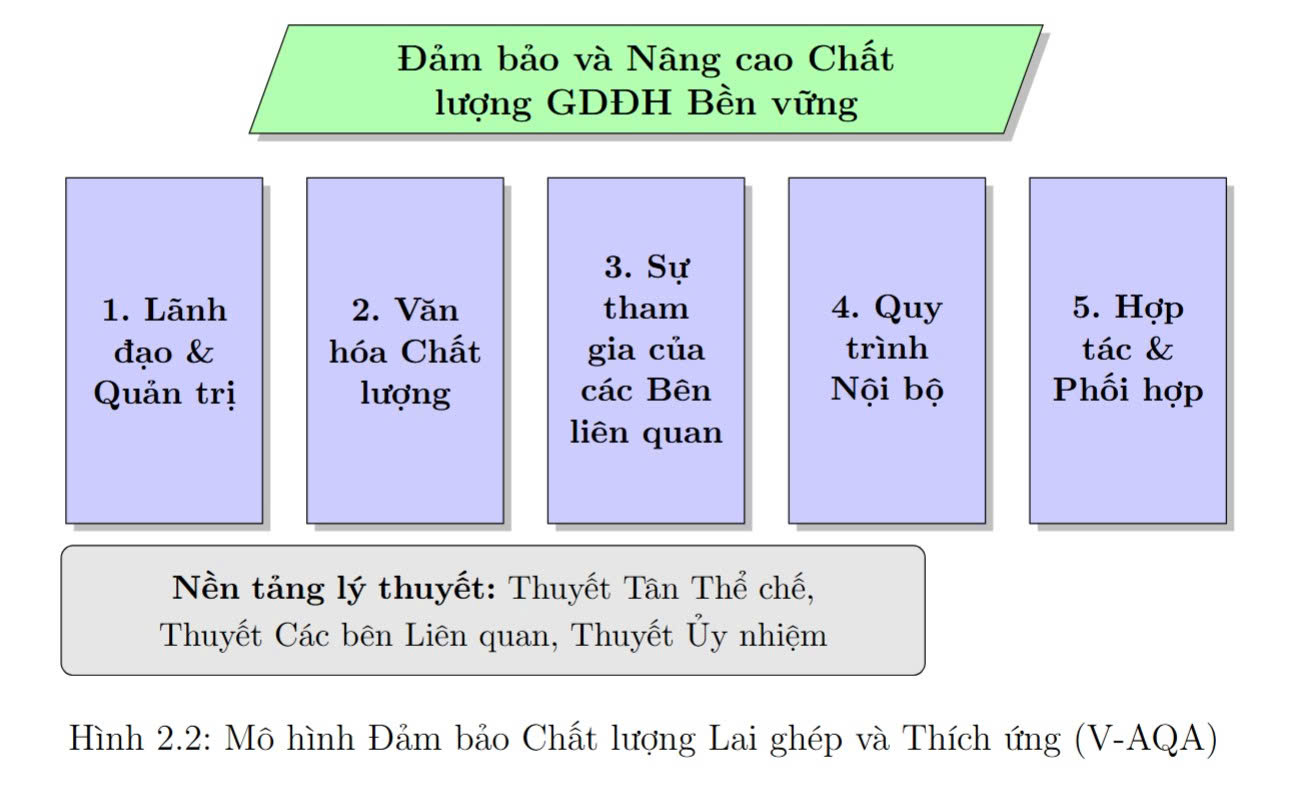
\includegraphics[width=\textwidth]{image/mo_hinh_V-AQA.jpg}
    \caption{混合与适应性质量保障模型 (V-AQA)}
    \label{fig:v-aqa-model-detailed}
\end{figure}

该系统需设计为能自动整合校内多个分散来源的数据,以创建关于质量的360度视图,包括:
\begin{itemize}
    \item \textbf{教学管理系统:} 学生数据、成绩、学习进度、辍学率。
    \item \textbf{人事系统:} 教师的学历、经验、专业发展活动和科研成果数据。
    \item \textbf{科技管理系统:} 研究课题、经费、科学论文数据。
    \item \textbf{在线调查系统:} 来自学生、教师、校友和雇主满意度调查的数据。
    \item \textbf{财务系统:} 用于教学、研究活动的预算分配和使用数据。
\end{itemize}

\paragraph{输出产品:智能报告与仪表盘。}
质量保障管理信息系统的最终目标不是存储数据,而是将数据转化为对各级决策有用的信息。为实现此目标,系统需配备一个\textbf{商业智能}模块,以自动生成可视化的报告和仪表盘,并为不同用户角色进行定制和授权\footcite{uq_kpi_dashboard}。

为更清晰地说明其可行性以及V-AQA模型如何通过数字工具运作,以下是为质量保障管理信息系统上不同角色定制的仪表盘示例。

\begin{table}[h!]
\centering
\caption{校长/校领导班子在质量保障管理信息系统上的关键绩效指标仪表盘示例}
\label{tab:dashboard_hieu_truong}
\begin{tabular}{|p{4.5cm}|p{2.5cm}|p{2.5cm}|p{2cm}|c|}
\hline
\textbf{战略指标(校级)} & \textbf{当前值} & \textbf{与上期比较} & \textbf{年度目标} & \textbf{状态} \\
\hline
12个月后学生就业率 & 92.5\% & $\blacktriangle$ 1.5\% & 95\% & 预警 \\
\hline
国际发表数量(Scopus/ISI) & 350 & $\blacktriangle$ 10\% & 400 & 达标 \\
\hline
雇主满意度 & 4.2/5 & $\blacktriangledown$ 0.1 & 4.5/5 & 未达标 \\
\hline
国际学生比例 & 8\% & $\blacktriangle$ 0.5\% & 10\% & 预警 \\
\hline
科研与技术转让收入 & 500亿 & $\blacktriangle$ 5\% & 600亿 & 预警 \\
\hline
\end{tabular}
\end{table}

\begin{table}[h!]
\centering
\caption{院长在质量保障管理信息系统上的关键绩效指标仪表盘示例}
\label{tab:dashboard_truong_khoa}
\begin{tabular}{|p{5cm}|p{2.5cm}|p{2.5cm}|p{2cm}|c|}
\hline
\textbf{运营指标(信息技术学院)} & \textbf{当前值} & \textbf{与上期比较} & \textbf{年度目标} & \textbf{状态} \\
\hline
按时毕业率 & 85\% & $\longleftrightarrow$ & 90\% & 预警 \\
\hline
学生对培养方案的满意度 & 3.9/5 & $\blacktriangle$ 0.2 & 4.2/5 & 预警 \\
\hline
院级科研课题数量 & 15 & $\blacktriangle$ 2 & 20 & 未达标 \\
\hline
参与培养方案改进的教师比例 & 60\% & $\blacktriangle$ 10\% & 80\% & 未达标 \\
\hline
\end{tabular}
\end{table}

\begin{table}[h!]
\centering
\caption{教师在质量保障管理信息系统上的关键绩效指标仪表盘示例}
\label{tab:dashboard_giang_vien}
\begin{tabular}{|p{5.5cm}|p{2.5cm}|p{3.5cm}|c|}
\hline
\textbf{个人指标(阮文A教师)} & \textbf{本学期} & \textbf{与全院平均比较} & \textbf{备注} \\
\hline
学生对教学的反馈得分 & 4.5/5 & +0.6 & 优秀 \\
\hline
已完成/计划科研时数 & 120/200 小时 & -40 小时 & 需改进 \\
\hline
学生课程通过率 & 95\% & +5\% & 良好 \\
\hline
专业发展活动 & 2门课程 & +1 & 良好 \\
\hline
\end{tabular}
\end{table}
    

部署一个质量保障管理信息系统不仅是一个技术解决方案,更是一场工作方式的改革。它要求领导层的坚定承诺、相应的资源投入,以及一个系统的培训计划,以使全体团队能够有效利用数据的力量。

\subsection{质量保障管理信息系统的风险分析与缓解方案}
\label{subsec:risk_qamis}
尽管带来巨大益处,部署质量保障管理信息系统也面临许多技术和人为风险。

\begin{itemize}
    \item \textbf{风险1:投资和维护成本超出能力。}
    \textit{表现:} 学校没有足够预算来构建、购买许可和维护一个复杂的信息系统。升级、维护和运营人员等隐性成本未被计算在内。
    \textit{缓解策略:}
    \begin{itemize}
        \item \textbf{分阶段实施:} 从最核心的模块开始,如学生数据管理和在线调查。更复杂的模块如商业智能将在证明其有效性后于后续阶段开发。
        \item \textbf{考虑开源解决方案:} 研究并利用开源平台以降低软件许可费用,将预算集中于定制和培训。
    \end{itemize}

    \item \textbf{风险2:数据不同步、不准确(垃圾进,垃圾出)。}
    \textit{表现:} 来自不同部门的数据在格式和可靠性上不一致。如果将“垃圾”数据输入系统,报告和分析将变得毫无意义。
    \textit{缓解策略:}
    \begin{itemize}
        \item \textbf{建立数据治理规定:} 颁布关于数据录入责任、格式标准化以及在集成到统一系统前对各部门数据进行检查、验证流程的明确规定。
        \item \textbf{投资于ETL(提取、转换、加载)过程:} 数据的清洗、转换和集成过程极其重要,需要投入相应的技术资源。
    \end{itemize}
    
    \item \textbf{风险3:来自最终用户的抵制。}
    \textit{表现:} 干部、教师不想使用新系统,因为它复杂、增加了工作量,或者他们感到被“监控”得太紧。
    \textit{缓解策略:}
    \begin{itemize}
        \item \textbf{设计友好的界面并关注用户利益:} 系统设计必须旨在帮助用户减少手工工作(例如:自动生成报告而非手动制作),而不仅仅是服务于管理层。
        \item \textbf{组织持续的培训和支持:} 建立一个支持团队(服务台),并提供直观易懂的指导材料。为特定用户群体组织实践培训。
    \end{itemize}
\end{itemize}

% het goi 7 chuong 4

























